\documentclass[compress]{beamer}
\usetheme{sthlm}

%-=-=-=-=-=-=-=-=-=-=-=-=-=-=-=-=-=-=-=-=-=-=-=-=
%        LOADING BEAMER PACKAGES
%-=-=-=-=-=-=-=-=-=-=-=-=-=-=-=-=-=-=-=-=-=-=-=-=

\usepackage{
booktabs,
datetime,
dtk-logos,
graphicx,
multicol,
pgfplots,
ragged2e,
tabularx,
tikz,
wasysym,
multirow,
float,
caption,
subcaption
}

\pgfplotsset{compat=1.8}

\usepackage[utf8]{inputenc}
\usepackage[portuguese]{babel}
\usepackage[T1]{fontenc}
\usepackage{newpxtext,newpxmath}
\usepackage{listings}

\lstset{ %
language=[LaTeX]TeX,
basicstyle=\normalsize\ttfamily,
keywordstyle=,
numbers=left,
numberstyle=\tiny\ttfamily,
stepnumber=1,
showspaces=false,
showstringspaces=false,
showtabs=false,
breaklines=true,
frame=tb,
framerule=0.5pt,
tabsize=4,
framexleftmargin=0.5em,
framexrightmargin=0.5em,
xleftmargin=0.5em,
xrightmargin=0.5em
}



%-=-=-=-=-=-=-=-=-=-=-=-=-=-=-=-=-=-=-=-=-=-=-=-=
%        LOADING TIKZ LIBRARIES
%-=-=-=-=-=-=-=-=-=-=-=-=-=-=-=-=-=-=-=-=-=-=-=-=

\usetikzlibrary{
backgrounds,
mindmap
}

%-=-=-=-=-=-=-=-=-=-=-=-=-=-=-=-=-=-=-=-=-=-=-=-=
%        BEAMER OPTIONS
%-=-=-=-=-=-=-=-=-=-=-=-=-=-=-=-=-=-=-=-=-=-=-=-=

\setbeameroption{show notes}

%-=-=-=-=-=-=-=-=-=-=-=-=-=-=-=-=-=-=-=-=-=-=-=-=
%        BEAMER COMMANDS
%-=-=-=-=-=-=-=-=-=-=-=-=-=-=-=-=-=-=-=-=-=-=-=-=


%-=-=-=-=-=-=-=-=-=-=-=-=-=-=-=-=-=-=-=-=-=-=-=-=
%
%	PRESENTATION INFORMATION
%
%-=-=-=-=-=-=-=-=-=-=-=-=-=-=-=-=-=-=-=-=-=-=-=-=

\title{Introdução a disciplina}
\subtitle{DCE540 - Computação Paralela e Distribuída}
%\date{\small{\jobname}}
\author{\texttt{Iago Carvalho}}
\institute{\texttt{Departamento de Ciência da Computação}}

\hypersetup{
pdfauthor = {Iago A. Carvalho},      
pdfsubject = {Computação Paralela e Distribuída},
pdfkeywords = {},  
pdfmoddate= {D:\pdfdate},          
pdfcreator = {WriteLaTeX}
}

\begin{document}

\begin{frame}
\titlepage

\end{frame}

%% --------------------------------------------------------

\begin{frame}{Computação Paralela}

Tradicionalmente, algoritmos são desenvolvidos para serem executados de forma linear.
\begin{itemize}
    \item Uma única instrução pode ser executada a cada vez.
    \item Após uma instrução, a próxima é executada.
\end{itemize}

\vspace{1cm}

Entretanto, uma forma comum de acelerar a execução de algoritmos é dividi-los em diversas pequenas partes.
\begin{itemize}
    \item Cada parte é resolvida de forma independente e simultânea.
    \item Os resultados de cada parte são agrupados para computar o resultado \textit{completo}.
\end{itemize}



\end{frame}

%% --------------------------------------------------------

\begin{frame}{Computação Paralela}

Computação paralela é altamente dependente de recursos de hardware.
\begin{itemize}
    \item Processadores multi-core
    \item Computadores multi-processador
    \item Processadores vetoriais (GPU)
    \item Clusters e grids computacionais
\end{itemize}

\vspace{0.5cm}

Computação Paralela pode ser classificada em quatro grandes tipos
\begin{itemize}
    \item Paralelismo em nível de bits
    \item Paralelismo em nível de instruções
    \item Paralelismo em nível de tarefas
    \item Paralelismo de \textit{loops} (\textit{Superworld Level Parallelism})
\end{itemize}
\end{frame}

%% --------------------------------------------------------

\begin{frame}{Paralelismo em nível de bits}

Processadores mais mordernos são capazes de manipular uma maior quantidade de informação.

\vspace{1cm}

Entre 1970 e 1990, processadores tinham uma palavra de 8 bits.
\begin{itemize}
    \item Adição de um inteiro de 8 bits por ciclo de clock
\end{itemize}

\vspace{1cm}

Processadores com tamanhos de palavra maiores surgiram
\begin{itemize}
    \item 16 bits $\rightarrow$ Adição de dois inteiros
    \item 32 bits $\rightarrow$ Adição de quatro inteiros
    \item 64 bits $\rightarrow$ Adição de oito inteiros
\end{itemize}

\end{frame}

%% --------------------------------------------------------

\begin{frame}{Paralelismo em nível de instruções}

\vspace{1cm}

\begin{figure}
    \begin{overprint}
    \onslide<1>\centering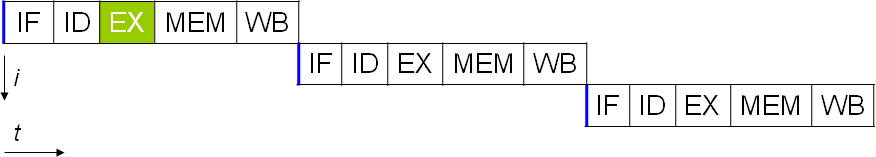
\includegraphics[width=0.80\textwidth]{images/serial.png}
    \onslide<2>\centering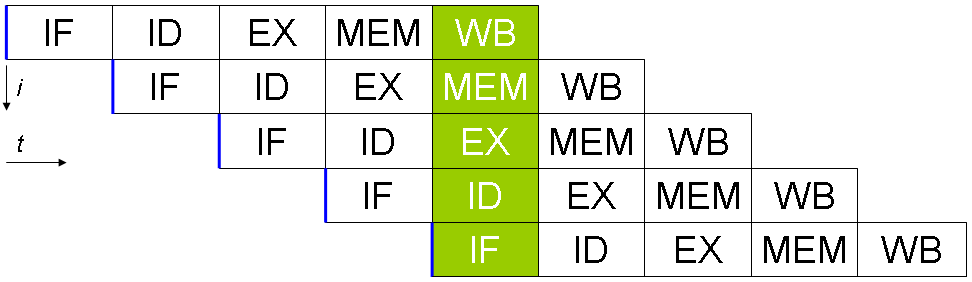
\includegraphics[width=0.80\textwidth]{images/pipeline.png}
    \end{overprint}
\end{figure}

\end{frame}

%% --------------------------------------------------------

\begin{frame}{Paralelismo de \textit{loops}}

\vspace{1cm}

\centering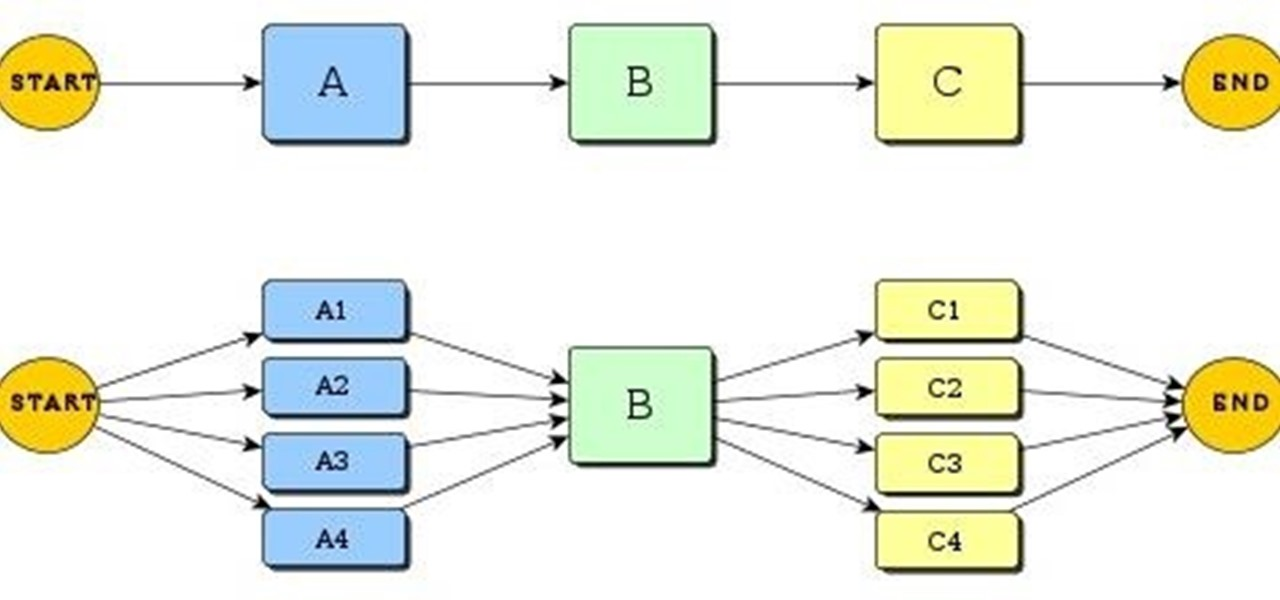
\includegraphics[width=0.80\textwidth]{images/parallel_for.jpg}

\end{frame}

%% --------------------------------------------------------

\begin{frame}{Computação Distribuída}

Sistemas distribuídos
\begin{itemize}
    \item Um sistema grande tem seus recursos localizados em diferentes dispositivos de rede
    \begin{itemize}
        \item Capacidade de processamento
        \item Bancos de dados
        \item Dispositivos de I/O
        \item Discos rígidos
    \end{itemize}
\end{itemize}

\vspace{0.5cm}

Um algoritmo que seja executado em um sistema distribuído é chamado de algoritmo distribuído.

\end{frame}

%% --------------------------------------------------------

\begin{frame}{Sistemas distribuídos}

As diversas partes de um sistema distribuído comunicam-se entre si utilizando mensagems
\begin{itemize}
    \item HTTP
    \item Remote Procedure Calls (RCP)
    \item Message Passing Interface (MPI)
    \item $\ldots$
\end{itemize}

\vspace{0.5cm}

Cada protocolo de mensagens tem um uso específico, em situações específicas.

Estas situações ficarão mais claras no decorrer deste curso.

\end{frame}

%% --------------------------------------------------------

%% --------------------------------------------------------

\begin{frame}{Aplicações}

\vspace{1cm}

\begin{figure}
    \begin{overprint}
    \onslide<1>\centering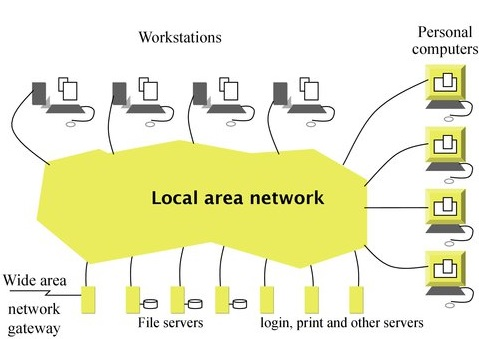
\includegraphics[width=0.80\textwidth]{images/laboratorio.jpg}
    \onslide<2>\centering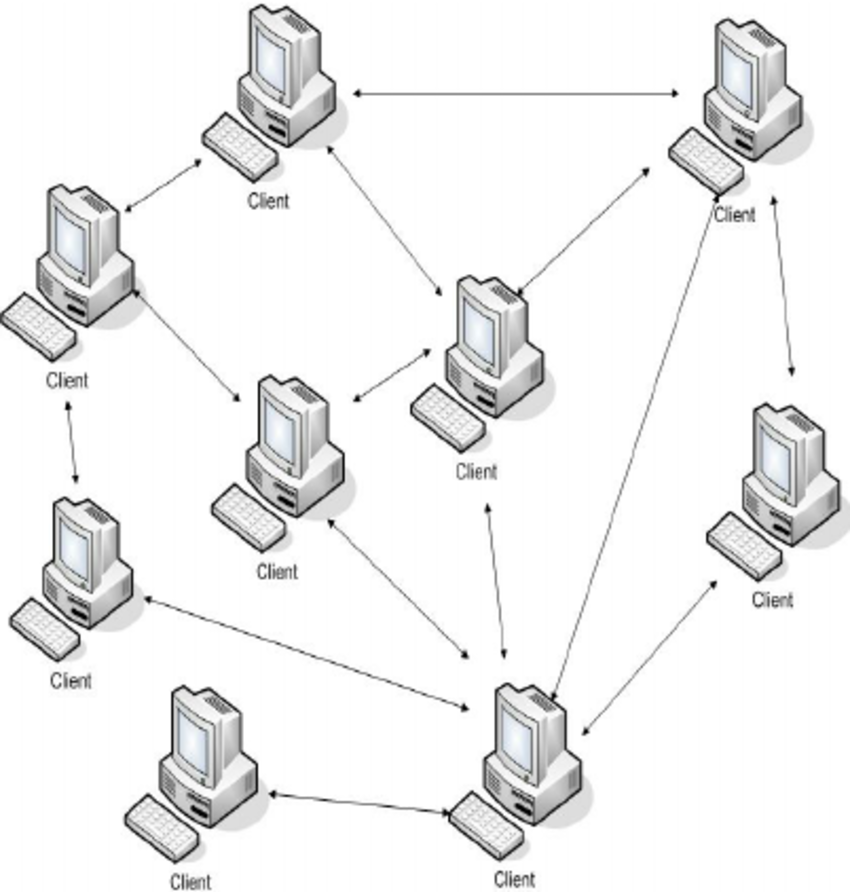
\includegraphics[width=0.63\textwidth]{images/p2p.png}
    \onslide<3>\centering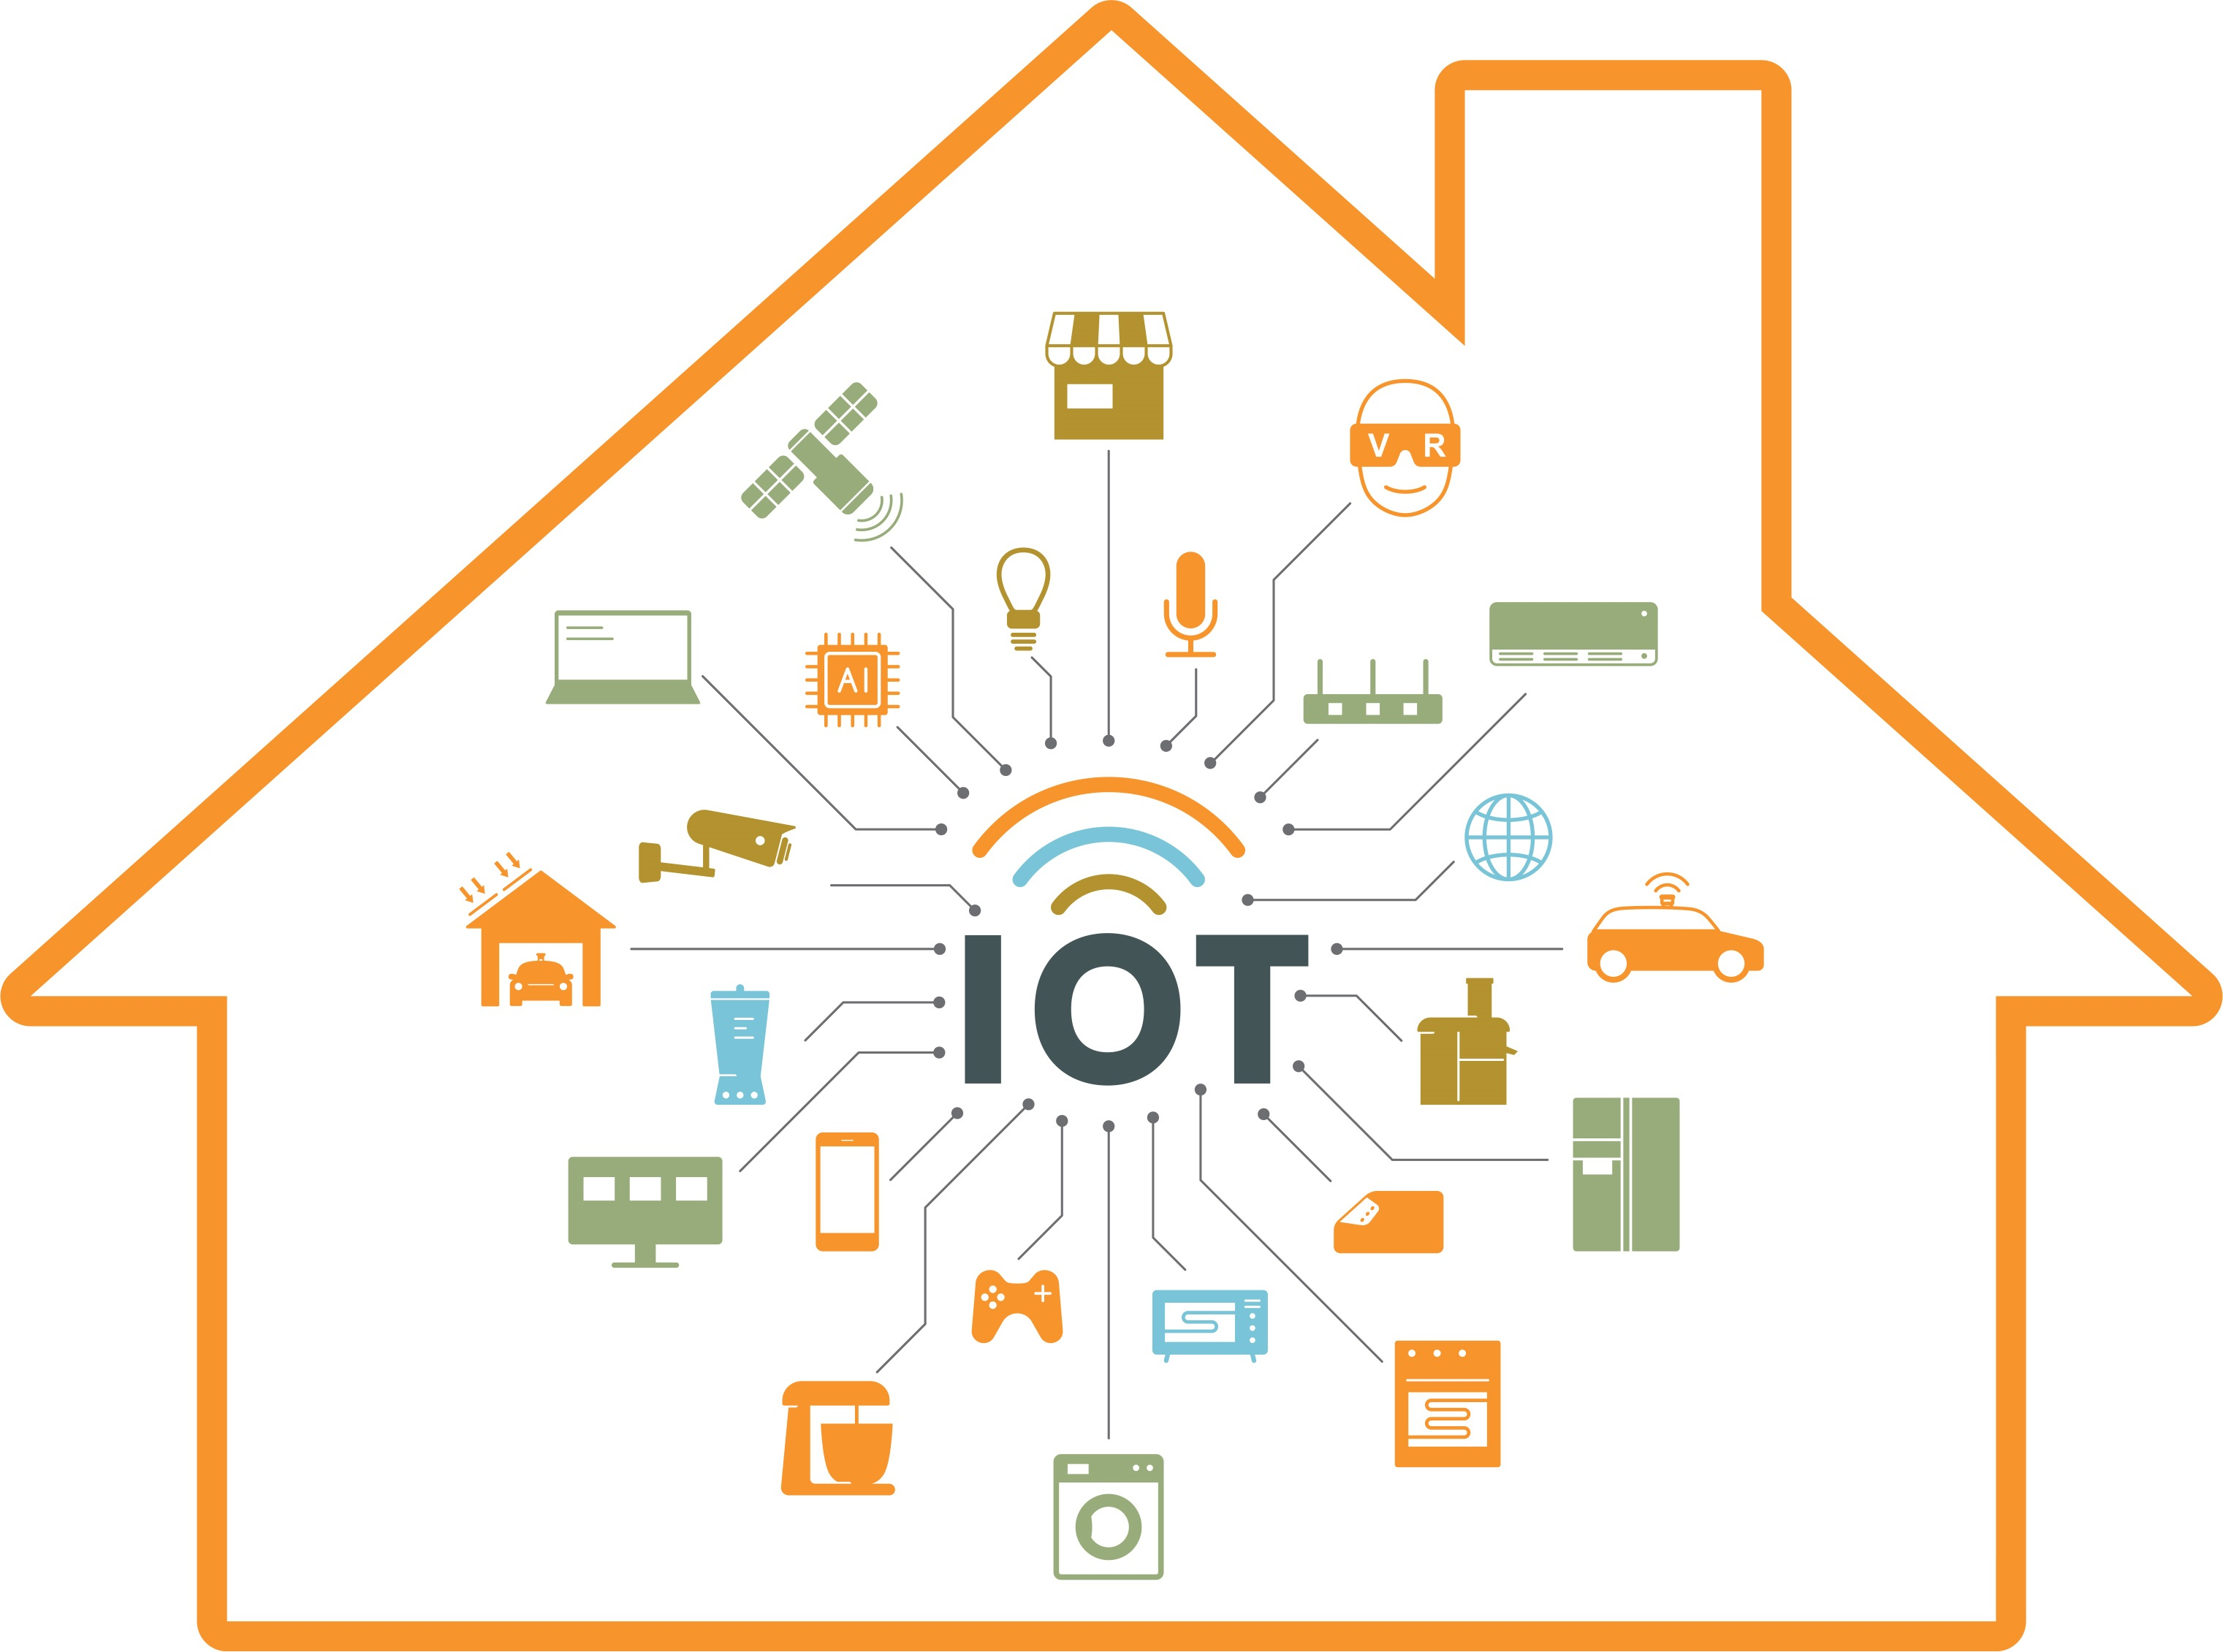
\includegraphics[width=0.80\textwidth]{images/iot.jpg}
    \onslide<4>\centering
\includegraphics[width=0.80\textwidth]{images/blockchain.png}
    \end{overprint}
\end{figure}

\end{frame}

\begin{frame}{Sobre a disciplina}

Página da disciplina no Github \href{https://github.com/iagoac/dce540}{\beamergotobutton{Link}}
\end{frame}

\end{document}